% Template for PLoS
% Version 1.0 January 2009
%
% To compile to pdf, run:
% latex plos.template
% bibtex plos.template
% latex plos.template
% latex plos.template
% dvipdf plos.template

\documentclass[10pt]{article}

% amsmath package, useful for mathematical formulas
\usepackage{amsmath}
% amssymb package, useful for mathematical symbols
\usepackage{amssymb}

% graphicx package, useful for including eps and pdf graphics
% include graphics with the command \includegraphics
\usepackage{graphicx}

% cite package, to clean up citations in the main text. Do not remove.
\usepackage{cite}

\usepackage{color} 

% Use doublespacing - comment out for single spacing
%\usepackage{setspace} 
%\doublespacing


% Text layout
\topmargin 0.0cm
\oddsidemargin 0.5cm
\evensidemargin 0.5cm
\textwidth 16cm 
\textheight 21cm

% Bold the 'Figure #' in the caption and separate it with a period
% Captions will be left justified
\usepackage[labelfont=bf,labelsep=period,justification=raggedright]{caption}

% Use the PLoS provided bibtex style
\bibliographystyle{plos2009}

% Remove brackets from numbering in List of References
\makeatletter
\renewcommand{\@biblabel}[1]{\quad#1.}
\makeatother


% Leave date blank
\date{}

\pagestyle{myheadings}
%% ** EDIT HERE **


%% ** EDIT HERE **
%% PLEASE INCLUDE ALL MACROS BELOW

%% END MACROS SECTION

\begin{document}

% Title must be 150 characters or less
\begin{flushleft}
{\Large
\textbf{Transcriptome variation in response to Marek's disease virus early infection}
}
% Insert Author names, affiliations and corresponding author email.
\\
Likit Preeyanon$^{1}$
C. Titus Brown$^{1,2}$
Hans H. Cheng$^{3,\ast}$
\\
\bf{1} Microbiology and Molecular Genetics, Michigan State University, East Lansing, MI, USA
\\
\bf{2} Computer Science and Engineering, Michigan State University, East Lansing, MI, USA
\\
\bf{3} USDA, ARS, Avian Disease and Oncology Laboratory, East Lansing, MI, USA
\\
$\ast$ E-mail: Corresponding hans.cheng@ars.usda.gov
\end{flushleft}

% Please keep the abstract between 250 and 300 words
\section*{Abstract}
Marek's disease (MD) is caused by highly oncogenic Marek's disease virus (MDV).
Different MHC alleles have been associated with susceptibility and resistance to the disease.
However, chickens line 6 and 7 show significant phenotypic differences when chanllenged with
MDV even with the same MHC allele. Therefore, the major unanswered question is what genetic factors
underlie the susceptibility and resistance of line 6 and 7.
In this study, we identified differentially expressed genes and isoforms in chicken line 6 and 7
in response to Marek's disease infection. Results from pathway analysis and functional analysis
show that changes in expression of genes and isoforms may contribute to resistance and
susceptibility of the disease. We also identified many single nucleotide polymorphisms (SNPs) between
line 6 and 7 that may cause alteration of alternative splicing, which in turn results in allele
specific expression.

% Please keep the Author Summary between 150 and 200 words
% Use first person. PLoS ONE authors please skip this step. 
% Author Summary not valid for PLoS ONE submissions.   
\section*{Author Summary}

\section*{Introduction}

Marek's disease is an economically significant chicken disease that affects a poultry industry worldwide.
Total of \$2 billion loss has been reported from outbreaks.
The disease is caused by highly oncogenic Marek's disease virus (MDV) which causes T-cell lymphoma.
Vaccination is effective in reducing incidence of tumor formation; however, current MD vaccines do not
prevent infection or horizontal spread of the virus.
Improper use of vaccines is a key factor that drives evolution of highly virulent strains in vaccinated
flocks.
***Need to add intro about breed selection against infection***

Many studies have reported strong associations between MHC alleles and resistance and susceptibility of
the disease. For example, chickens with MHC allele B$^{21}$ is highly resistant in contrast to chickens with
B$^{16}$ allele.
However, chickens line 6 and 7 , even with common allele (B$^6$), exhibit different phenotypic response to
MD.
The major unanswered question is what genetic factors contribute to susceptibility and resistance of
the disease.
***Need to add intro about gene and isoforms in immune system***
In this study, we identified several annotated and unannotated genes and isoforms that are differentially
expressed in response to MD infection. Pathway analysis and gene ontology suggest that these
genes may have important roles in immune response to MD.


% Results and Discussion can be combined.
\section*{Results}

\subsection*{Custom Gene Annotations}
A large number of reads mapped to intergenic and intronic regions (table 1, supp.)
regions of Ensembl annotations (Galgal4.72)
indicates that many genes and isoforms are not included in the annotations.
Therefore, to extensively study gene and isoform expression, we employed \emph{de novo}
transcriptome assembly as well as genome-based assembly to build custom gene annotations (see methods).
The number of genes and isoforms is shown in Table \ref{tab:gene_models}.
Genes were identified by aligning against all vertebrate transcripts in GenBank database.
We found several genes that not annotated in either RefSeq or Ensembl, including chicken specific genes
as well as genes found in other organisms (Table \ref{}).


\subsection*{Differential Gene Expression}
Many previous studies have reported many differentially expressed (DE) genes between line 6 and line 7
from Microarray and RNA-Seq experiments from different stages of infection.
Some known differentially expressed genes were identified in this study.
For example, B6.1 (Bu-1) gene is known to be down-regulated approximately 2.5 fold in susceptible
chicken with MHC allele B\textsuperscript{19}\cite{}. It was also found to be down-regulated
about three fold in line 7.

Even though both lines shared a significant number of genes that were differentially expressed,
approximately, twice as many genes in line 7 as in line 6 were differentially expressed (Table \ref{tab:dge}).
Interestingly, some genes that were differentially expressed in both lines were
regulated in opposite directions.
As shown in table \ref{tab:opposite}, LYG2, SFTPA1, LL and SERPINB10 were up-regulated in line 7 but down-regulated in line 6.
In contrast, TAF1D and LOC424145 were up-regulated in line 6 but down-regulated in line 7.
LYG2, for instance, was up-regulated by 2.57 folds in line 7 but down-regulated by 1.7 folds in line 6.
This gene is involved in a defense against bacteria.

Pathway analysis shows that genes in line 7 are significantly enriched (p $< 0.05$) in pathways involved in
immune system such as Toll-like receptor signaling, intestinal immune network for IgA production,
and Phagosome pathway, which are not significantly enriched in line 6 (fig. \ref{line67_kegg}).
Figure \ref{KEGG_phagosome} and \ref{KEGG_IgA} shows a diagram of phagosome and intestinal immune network
for IgA production repectively. Genes from line 6 and line 7 are highlighted with yellow and red color.
Common genes are highlighted with orange color.
These two pathways show that both line 6 and line 7 regulated MHC class I gene in response to infection,
but only line 7 regulated MHC class II gene.
It has been shown that Marek's disease virus (MDV), unlike other herpes viruses, up-regulates MHC class II gene
during infection. Moreover, regulation is believed to be mediated directly by MDV infection\cite{Niikura:2007fq}.
However, from these results, it appears that only MHC class II gene in line 7 was up-regulated.

Furthermore, differentially expressed genes in line 7 are enriched in biological processes involved in
both adaptive and innate immune responses, whereas
differentially expressed genes in line 6 are only enriched in innate immune responses (fig. \ref{line67_go}).
This might correspond to the fact that MHC class II gene was upregulated in line 7.
High level of MHC class II molecules may help recruit more T cells, which in turn enhance activation of
the adaptive immune response.


\subsection*{Differential Exon Usage}

\subsection*{Functional Analysis}
\subsection*{Polymorphisms in differentially expressed genes/exons}


\section*{Discussion}

% You may title this section "Methods" or "Models". 
% "Models" is not a valid title for PLoS ONE authors. However, PLoS ONE
% authors may use "Analysis" 
\section*{Materials and Methods}
\subsection{Gene Models Construction}
With the lack of high quality gene models for chickens. We employed two different approaches to
construct gene models from RNA-Seq reads.
First, short reads were quality trimmed with conditri/2.1\cite{} \texttt{(-cutfirst 10)}
and assembled using Velvet/1.21\cite{} and Oases/0.2.06\cite{} to obtain long transcripts.
Assembly was done with k value ranges from 21 to 31 for both local and global assembly
(described in Gimme paper\cite{}).
Poly-A tails were trimmed and low complexity transcripts were removed by Seqclean\cite{}.
All transcripts were then aligned to chicken reference genome (galGal4, with short
contigs removed) with BLAT\cite{} \texttt{(-t=dna -q=dna -noHead -out=psl -mask=lower -extendThroughN)}.
Filtered alignments from BLAT were then used to produced gene models using Gimme.

Second, short reads were aligned to reference genome using Tophat/2.0.5\cite{} and mapping output were used to
build gene models by Cufflinks2\cite{} with default parameters.
Both set of gene models were combined using Gimme to build more comprehensive models
to be used in this study.

\subsection{Differential Gene Expression and Gene Ontology}

To identify DE genes, we obtained read counts using multiBamCov command from BEDTools/12.13.1\cite{}
for all datasets.
Then DE gene were identified by DESeq/1.10.1\cite{S:2010fu} from Bioconductor.
Data from single- and paired-end datasets from the same line were treated as biological replicates.
To identify enriched pathways and ontology terms, a list of DE genes was analysed by GOSeq/1.10.0\cite{}.
P-values were corrected by Benjamini-Hochberg multiple testing correction.
Genes, patways and GO terms with corrected P-value $<0.05$ were considered significant.

\subsection{Differential Splicing Event}
Gene models were converted to alternative splicing models using a Python script.
In order to increase sensitivity, read counts from single- and paired-end samples were combined and treated
as single-end reads for splicing event analysis with MISO/0.4.9\cite{Katz:2010iv}.
Splicing events with Bayes factor $>10$ and $\Delta\Psi>0.20$ were considered significant.
Read coverages and $\Psi$ distributions were plotted using Sashimi plot\cite{Katz:2013vx}.

\subsection{Variant Calling and \emph{In Silico} Splicing Analysis}
Variants were called using mpileup command from SAMTools/0.1.18\cite{} and BCFTools\cite{}.
Only variants with quality score $\ge20$ were used for mutation analyses.
Exon enhancers and suppressors were predicted using Human Splicing Enhancer web portal\cite{}.
Human default parameter settings were used in all analyses.
The following regulatory sequences were used to determined the effect of variants:
HSF integrated matrices for serine/arginine-rich proteins (SRp40, SC35, SF2/ASF, SF2/ASF,
IgM/BRCA1, and SRp55), exonic splicing enhancer (ESE), RESCUE-ESE hexamer (RESCUE-ESE),
putative 8-mer ESEs (PESEs) and putative 8-mers exonic splicing silencers (PESSs),
exon-identity and intron-identiry elements (EIEs and IIEs), hetronuclear ribonucleoprotein-binding
motifs, and Fas exonic splicing silencers.

% Do NOT remove this, even if you are not including acknowledgments
\section*{Acknowledgments}

% \section*{References}
% The bibtex filename
\bibliography{ref}{}

\section*{Figure Legends}
\begin{figure}[!ht]
\begin{center}
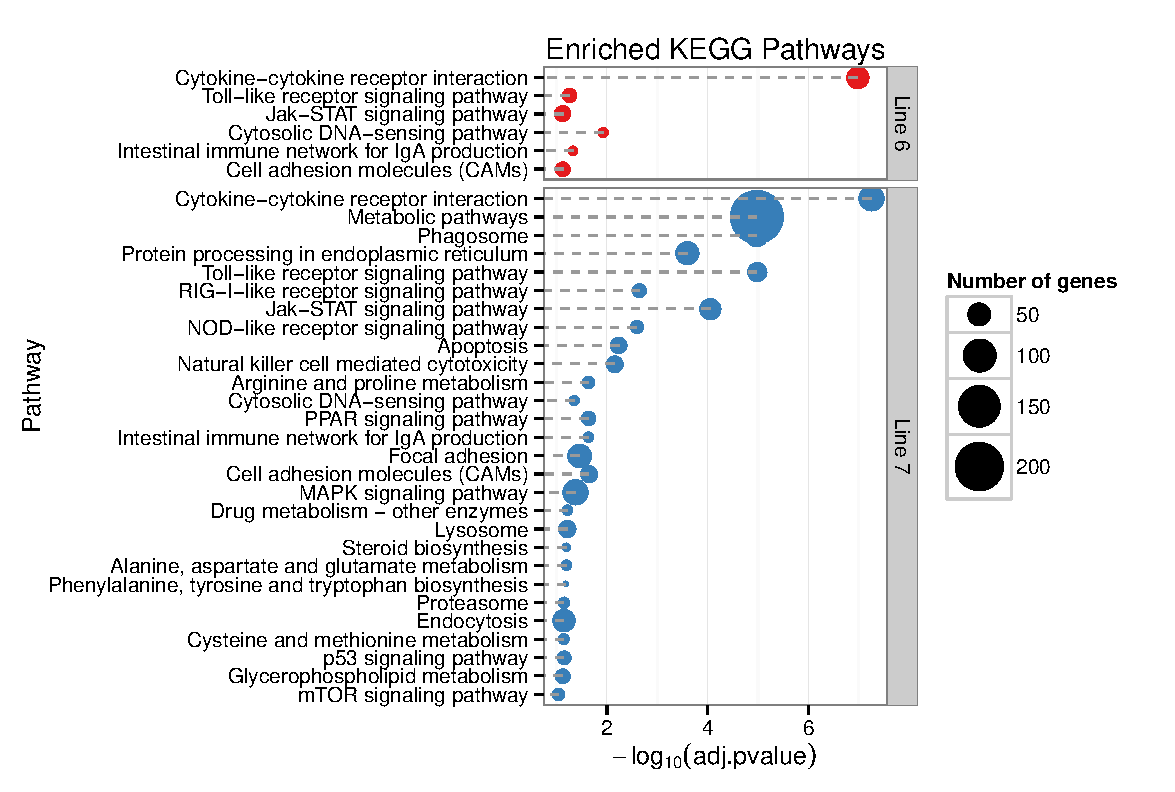
\includegraphics[width=7in]{line67_KEGG_cleveland.pdf}
\end{center}
\caption{
{\bf Enriched KEGG pathways.} Rest of figure 2  caption.  Caption 
should be left justified, as specified by the options to the caption 
package.
}
\label{line67_kegg}
\end{figure}

\begin{figure}[!ht]
\begin{center}
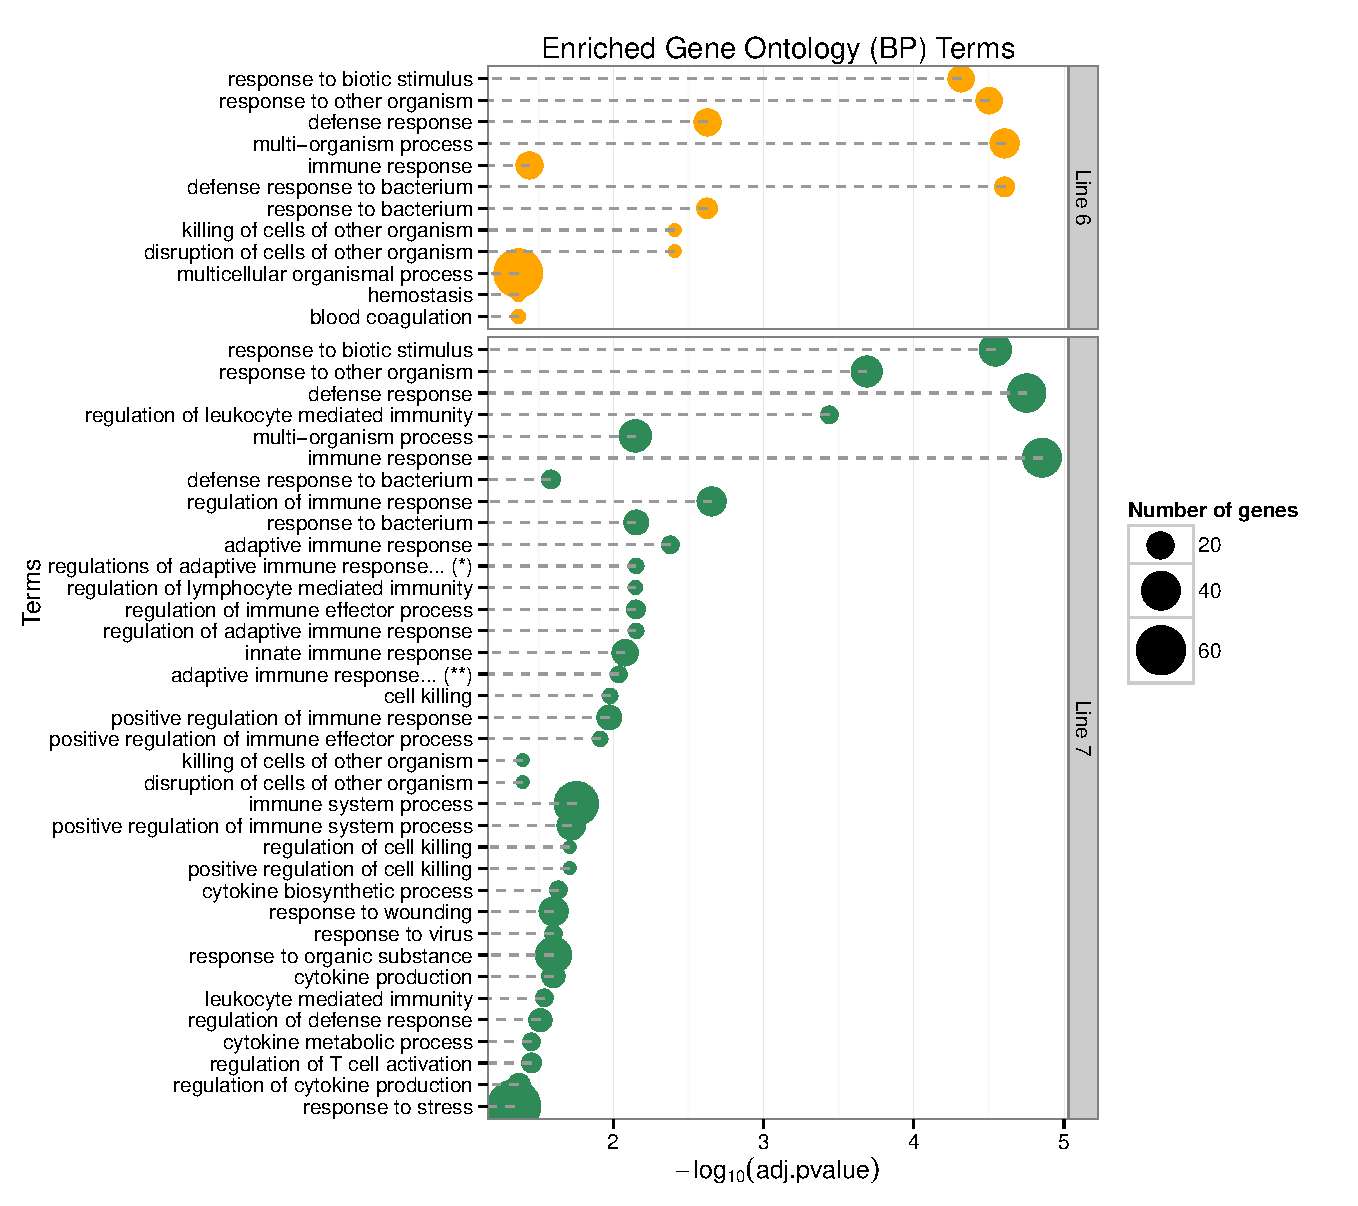
\includegraphics[width=7in]{line67_GOseq_GO_cleveland.pdf}
\end{center}
\caption{
{\bf Enriched Gene Ontology (BP) Terms.} Rest of figure 2  caption.  Caption 
should be left justified, as specified by the options to the caption 
package.
}
\label{line67_go}
\end{figure}

\begin{figure}[!ht]
\begin{center}
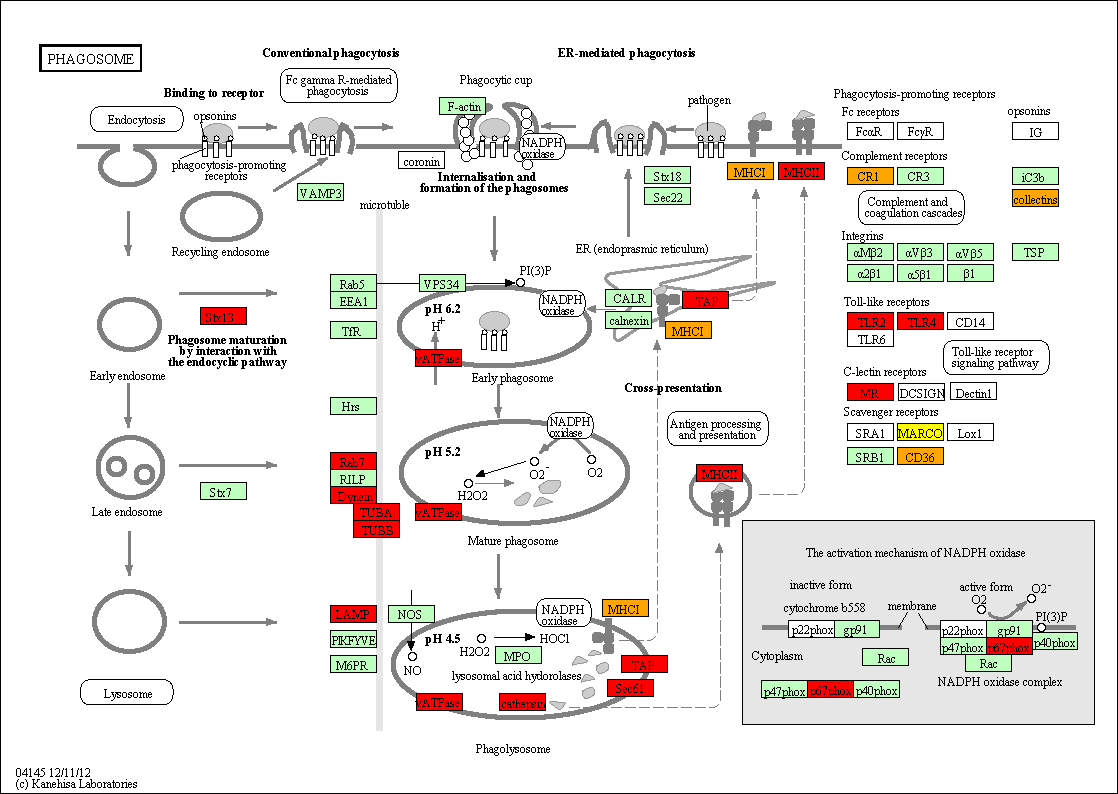
\includegraphics[width=6in]{line67_KEGG_gga04145.png}
\end{center}
\caption{
{\bf Enriched KEGG pathways in line 7.}  Rest of figure 2  caption.  Caption 
should be left justified, as specified by the options to the caption 
package.
}
\label{KEGG_phagosome}
\end{figure}

\begin{figure}[!ht]
\begin{center}
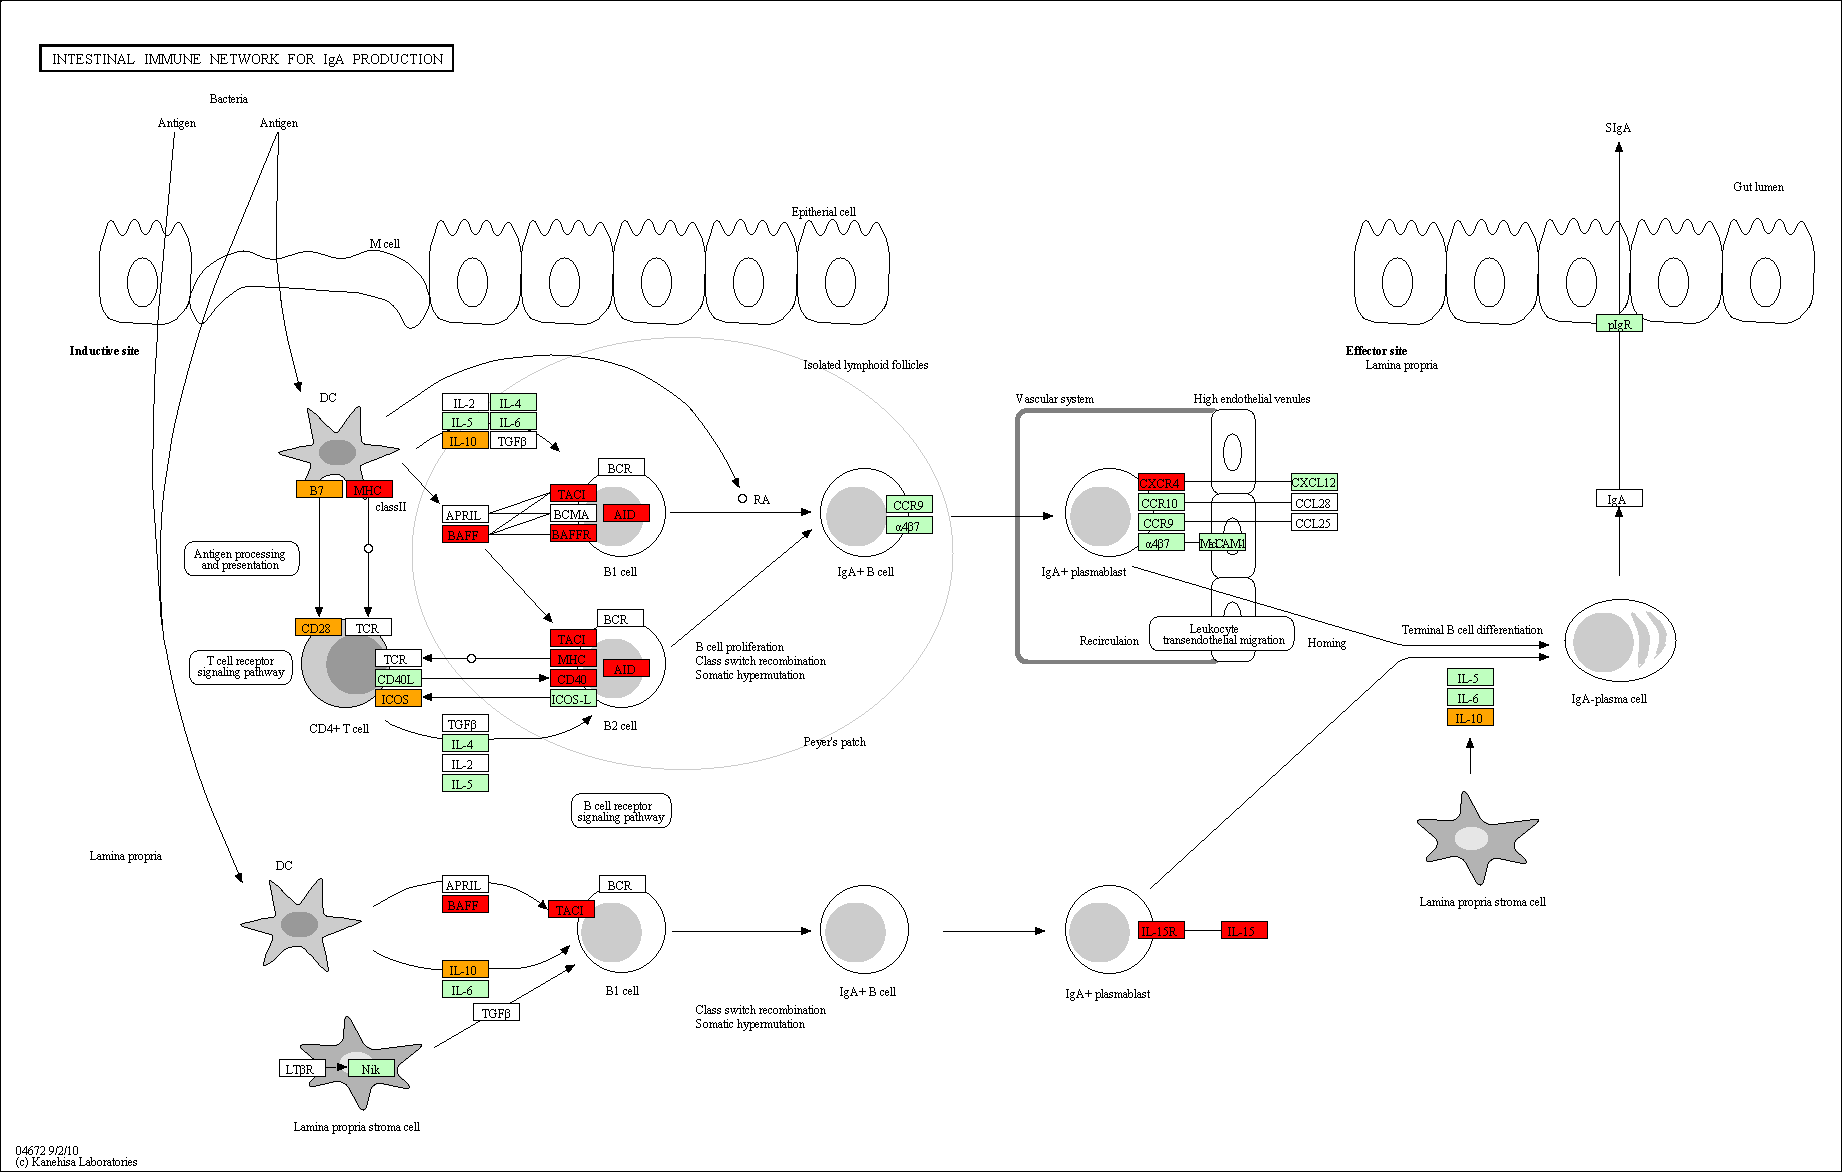
\includegraphics[width=6in]{line67_KEGG_gga04672.png}
\end{center}
\caption{
{\bf Intestinal network for IgA production pathway.}  Rest of figure 2  caption.  Caption 
should be left justified, as specified by the options to the caption 
package.
}
\label{KEGG_IgA}
\end{figure}

\section*{Tables}

\begin{table}[!ht]
\caption{
\bf{Gene models summary}}
\begin{tabular}{ccc}
\hline
Method & Gene & Isoform \\
\hline
Assembly & 25,290 & 54,044 \\
Cufflinks & 21,345 & 36,218 \\
Combined & 24,980 & 46,613 \\
\hline
\end{tabular}
\begin{flushleft}Number of genes and isoforms from gene models
built from \emph{de novo} assembly and Cufflinks.
Combination of both methods decreased the number of genes
and isoforms by merging fragmented transcripts to
form more complete gene models.
\end{flushleft}
\label{tab:gene_models}
\end{table}

\begin{table}[!ht]
\caption{
\bf{Differentially expressed genes}}
\begin{tabular}{cccccc}
\hline
Sample & Up-regulated & Down-regulated & Total & Refseq & Ensembl\\
\hline
Line 6 & 1,043 & 595 & 1,188 & 984 (60.0\%) & 1,252 (76.4\%) \\
Line 7 & 1,976 & 1,124 & 3,100 & 2,114 (68.2\%) & 2,574 (83.0\%) \\
Both & 681 & 236 & 917 & 664 (72.4) & 771 (84.1\%) \\
\hline
\end{tabular}
\begin{flushleft}
    FDR $< 0.1$
\end{flushleft}
\label{tab:dge}
\end{table}

\begin{table}[!ht]
\caption{
\bf{Genes regulated in opposite direction}}
\begin{tabular}{cccccc}
\hline
Gene & Entrez ID & Fold Change & \\
 & & Line 6 & line 7 \\
\hline
TAF1D & 419002 & +1.08 & -1.13 \\
LYG2 & 395708 & -1.70 & +2.57 \\
SFTPA1 & 395308 & -5.12 & +3.51 \\
LOC424145 & 424145 & +1.57 & -1.68 \\
LL & 423630 & -3.30 & +8.31 \\
SERPINB10 & 395715 & -1.12 & +0.87 \\
\hline
\end{tabular}
\begin{flushleft}
    (-) down-regulated, (+) up-regulated
\end{flushleft}
\label{tab:opposite}
\end{table}
\end{document}

